\documentclass[10pt,a4paper]{beamer}
\usepackage[utf8]{inputenc}
\usepackage[T1]{fontenc}
\usepackage[francais]{babel}
\usepackage{amsmath}
\usepackage{amsfonts}
\usepackage{hyperref}
\usetheme{Warsaw}

\subtitle{Développement Web sur le framework Ruby on Rails}
\title{Soutenance Intermédiaire}
\author{Jaussoin Timothée \\ \and Maitre de Stage Floris Vlasveld \\ \and Enseignant Responsable Normand Nicolas}
\institute{Polytech Nantes - Département Informatique}

\begin{document}
\begin{frame}
  \titlepage
\end{frame}

\begin{frame}{About the internship}
  \begin{itemize}
    \item 6 months
    \item Inspire, Utrecht, The Netherlands
  \end{itemize}
  
  \section{About the Internship}
  
  \begin{block}{Topic}
    \begin{itemize}
      \item Web Development on Ruby on Rails
      \item Frontend oriented (Javascript, HTML5, CSS)
    \end{itemize}
  \end{block}

  \begin{block}{Project}
    \begin{itemize}
      \item Calibris - Questionnaire Manager
      \item Add new features, refactor and optimize the source-code
    \end{itemize}
  \end{block}
\end{frame}

\section{Calibris}
\subsection{Overview}

\begin{frame}{Calibris - Overview}

  \begin{figure}[htp]
  \centering
  
\includegraphics[scale=.50]{../img/calibris.jpg}
   \caption{Calibris Logo}
  \end{figure}
  
  \begin{itemize}
    \item Rails application
    \item Now used by several clients
  \end{itemize}

  \begin{block}{Features}
    \begin{itemize}
      \item Manage organizations (with 3 roles)
      \item Manage questionnaires (import, link)
      \item Manage surveys (create, organize, send emails)
    \end{itemize}
  \end{block}
\end{frame}

\begin{frame}{Calibris - Overview}
  \begin{figure}[htp]
  \centering
  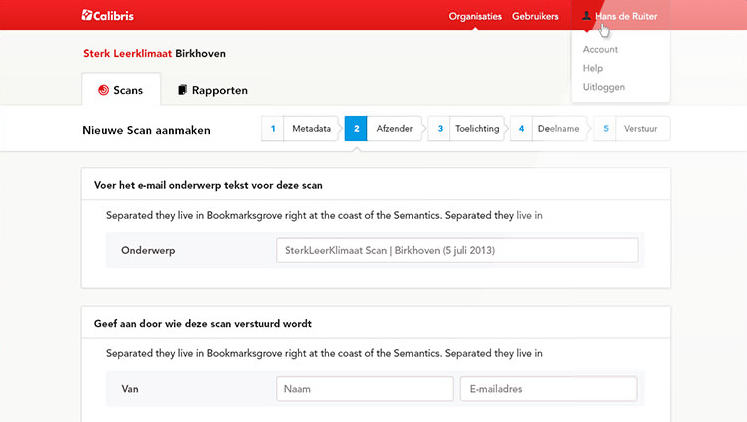
\includegraphics[scale=0.4]{../img/calibris1.png}
   \caption{Creating a new survey on Calibris}
   \label{fig.calibris1}
  \end{figure}
\end{frame}
  
\begin{frame}{Calibris - Overview}
  \begin{figure}[htp]
  \centering
  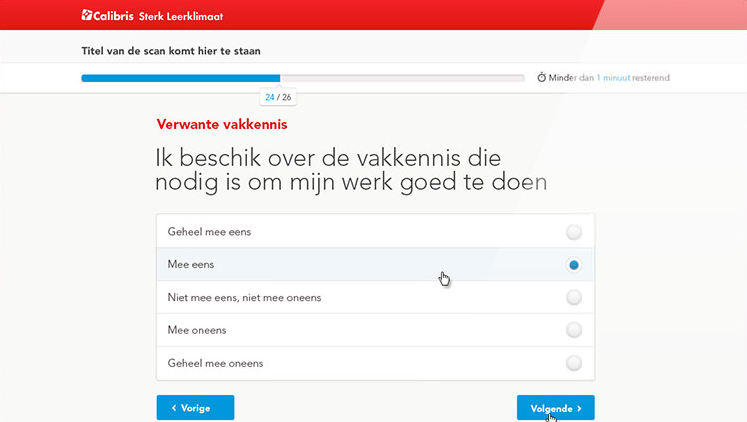
\includegraphics[scale=0.4]{../img/calibris2.png}
   \caption{Aswering a questionnaire on Calibris}
   \label{fig.calibris2}
  \end{figure}
\end{frame}

\subsection{Projects}

\begin{frame}{Projects}
  \begin{description}
    \item[Project 1] Questionnaire Manager
    \item[Project 2] Update to Rails 4.1
    \item[Project 3] Mobile version
    \item[Project 4] Survey refactor
  \end{description}
  But also… fixing issues and participating with the team in the daily updates and improvements of Calibris.
\end{frame}

\subsubsection{Questionnaire Manager}

\begin{frame}{Questionnaire Manager}
  \begin{block}{Questionnaires structure}
    \begin{itemize}
      \item Categories
      \item Clusters
      \item Questions 
    \end{itemize}
  \end{block}

  \begin{block}{To Do}
    \begin{itemize}
      \item Implement basic CRUD (Create, Read, Update and Delete) actions 
      \item Add inline editing
      \item Add drag\&drop reordering 
      \item Link it with the all application
    \end{itemize}
  \end{block}
  
  \begin{block}{}
    \begin{itemize}
      \item 8 weeks
      \item Merged in the trunk
    \end{itemize}
  \end{block}
\end{frame}

\begin{frame}{Questionnaire Manager - Implementation}
  \begin{itemize}
    \item Using \texttt{awesome\_nested\_set} to handle the questionnaires structures
    \item Using the Rails \texttt{remotes} tu send and receive dynamicaly parts of the page
    \item Using jQuery sortable to reorder dynamicaly the categories, clusters and questions
  \end{itemize}
  
  \begin{figure}[htp]
  \centering
  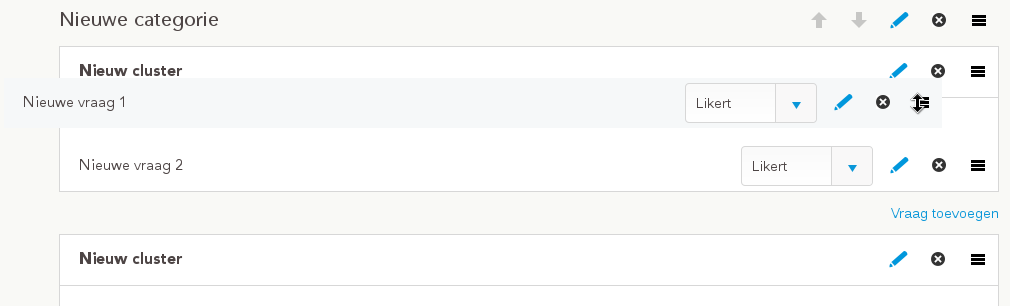
\includegraphics[scale=0.3]{../img/calibris_drag_drop.png}
   \caption{Drag\&Drop a question}
  \end{figure}
\end{frame}

\subsubsection{Rails 4.1 Upgrade}

\begin{frame}{Rails 4.1 Upgrade}
  \begin{block}{To Do}
    \begin{enumerate}
      \item Update the Gemfile
      \item Fixing the critical bugs
      \item Running the test suite
      \item Fixing the remaining bugs
    \end{enumerate}
  \end{block}
  
  \begin{block}{}
    \begin{itemize}
      \item 3 weeks
      \item Trunk updated
    \end{itemize}
  \end{block}
\end{frame}

\subsubsection{Mobile version}

\begin{frame}{Mobile version}
  \begin{block}{To Do}
    \begin{itemize}
      \item Make the CSS responsive (using CSS3 media-queries)
      \item Check on desktop 
      \item Check the size and resolution of the elements
      \item Check on iOS, Android
      \item Fix the remaining issues 
    \end{itemize}
  \end{block}
  
  \begin{block}{}
    \begin{itemize}
      \item 1-2 weeks + minor issues
      \item Merged in the trunk
    \end{itemize}
  \end{block}
\end{frame}

\begin{frame}

\begin{figure}[htp]
\centering
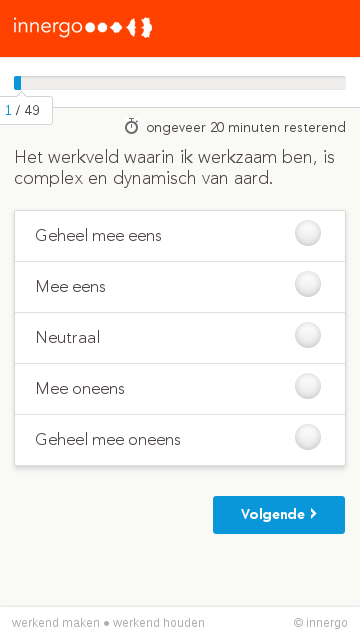
\includegraphics[scale=0.32]{../img/calibris3.png}
 \caption{The respondents view on mobile}
 \label{fig.calibris3}
\end{figure}

\end{frame}

\subsubsection{Survey Refactor}

\begin{frame}{Survey Refactor}
  \begin{quotation}
    \Large ``The weak part of the application''
  \end{quotation}

  \begin{block}{To Do}
    \begin{itemize}
      \item Understand how a survey is currently created (blackbox system)
      \item Recreate a simple form that do quite the same thing
      \item Add some Javascript and CSS
      \item Fix the tests and be sure that all works correctly
    \end{itemize}
  \end{block}
  
  \begin{block}{}
    \begin{itemize}
      \item Already 2 weeks
      \item No merged yet
    \end{itemize}
  \end{block}
\end{frame}

\section{Summary}

\begin{frame}{Summary}
    \begin{block}{Skills}
    \begin{itemize}
      \item Rails environment comprehension
      \item Frontend technologies (Javascript, CSS3)
      \item Organisation (Jira, Agile)
      \item Code management (Git, GitHub)
    \end{itemize}
  \end{block}
  
  \begin{itemize}
    \item Calibris, a full stack Rails project 
    \item Daily improvements and fixes
    \item Blog post
  \end{itemize}
\end{frame}

\end{document}